% Tento soubor nahraďte vlastním souborem s obsahem práce.
%=========================================================================
% Autoři: Michal Bidlo, Bohuslav Křena, Jaroslav Dytrych, Petr Veigend a Adam Herout 2019

% Pro kompilaci po částech (viz projekt.tex), nutno odkomentovat a upravit
%\documentclass[../projekt.tex]{subfiles}
%\begin{document}

\chapter{Úvod}
%cca strana

\chapter{Teoretická část} %přejmenovat

\section{Hardware Adeept AWR 4WD a Raspberry Pi 4}
Celá práce je implementována nad existujícím hardwarem. Konkrétně se jedná o "stavebnici" Adeept AWR 4WD z níž pochází všechny periferie, jako motory, serva a čidla. Tyto periferie jsou pak ovládány mikropočítačem Raspberry Pi4 ve verzi s 4GB operační paměti. V porovnání s běžně používanými mikrokontrolery se jedná o výkonější hardware.

\subsection*{Raspberry Pi}


\subsubsection{Ubuntu Server}
Jako operační systém na němž celý systém poběží byl zvolen 64-bitový Ubuntu server.

\subsection*{Adeept AWR 4WD}

\subsubsection*{Robot HAT}
Adeept Robot HAT je hardwarová deska, která slouží k rozšíření Rapsberry Pi o další funkcionalitu. K rpi se připojuje pomocí GPIO(General purpuse input outpu) pinů. Deska jako taková obsahuje rozšiřující čipy a rozhraní sloužící k ovládání připojených periferií.

\begin{itemize}
	\item{PCA9685 \cite{pca9685}}
	\begin{itemize}
		\item{generátor PWM signálu}
		\item{16 kanálů}
		\item{12 bitů rozlišení střídy (4096 možných hodnot)}
		\item{je ovládaný přes I2C sběrnici}
	\end{itemize}
	\item{L298P}
	\begin{itemize}
		\item{ovladač pro řízení dc motoru}
		\item{obsahuje full bridge obvod (viz následující obrázek)}
		\item{umožňuje roztočit motor oběma směry}
		\item{pomocí PWM lze ovládat rychlost motorů}
	\end{itemize}
\end{itemize}

\begin{figure}[h!]
	\centering
	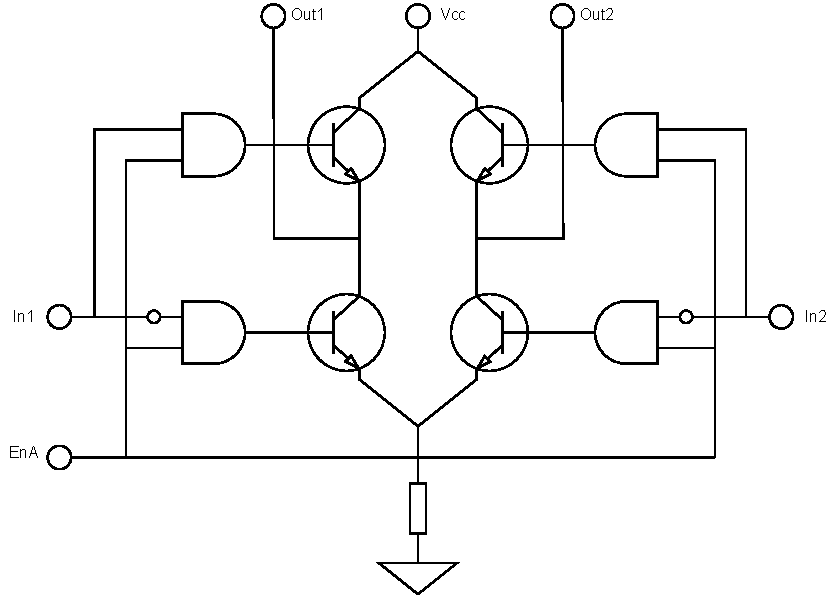
\includegraphics[scale=0.75]{obrazky-figures/motor_full_bridge.pdf}
	\caption{Full bridge konfigurace pro ovládání motoru. In1 a In2 určují směr otáčení. EnA je PWM signál určující rychlost otáčení. \cite{l298}}
	\label{}
\end{figure}

%batery - napájení

\subsubsection{I2C}
Je synchronní sběrnice, která se vyznačuje svou jednoduchostí a nízkou cenou. Využívá dva vodiče SDA (serial data) a SCL (serial clock). Oba vodiče jsou připojeny k napájecímu napětí pomocí pull-up rezistoru a bez vlivu jiného hardwaru zůstávají v logické jedničce. Zařízení která jsou na tuto sběrnici připojeny využívají open drain k úpravě aktuální napěťové úrovně na sběrnici. I2C pak pracuje s dvěma druhy zařízení, master a slave. Master zahajuje a ukončuje komunikaci, typicky se jedná o mikrokontroler. Slave jsou pak ostatní zařízení s nimiž může master komunikovat, typicky různé periferie. \cite{um10204}

\begin{figure}[h!]
	\centering
	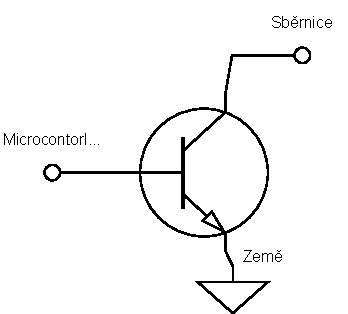
\includegraphics[scale=0.75]{obrazky-figures/open_drain.pdf}
	\caption{Open drain}
	\label{}
\end{figure}

Přenos jednoho datového rámce zahájí master zařízení přivedením datové sběrnice do nuly. Následující komunikace se skládá z odeslání rámce o délce osmi bitů a potvrzení o úspěšném přenosu dat od přijímajícího zařízení. Toto potvrzení se nazývá ACK a je provedeno podržením datové sběrnice v hodnotě nula po dobu jednoho taktu. Opačný stav se nazývá NACK a indikuje že došlo k chybě. Ukončení přenosu je provedeno navrácením datové sběrnice na hodnotu jedna.

\begin{figure}[h!]
	\centering
	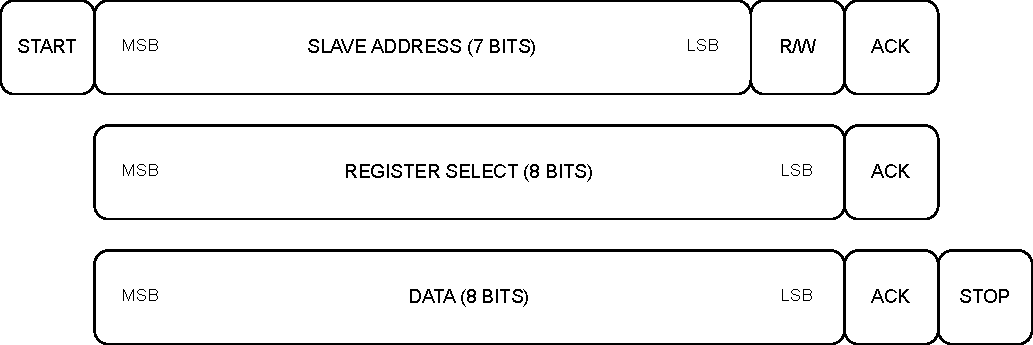
\includegraphics[scale=0.75]{obrazky-figures/i2c_data_word.pdf}
	\caption{Na obrázku lze vidět, jak může vypadat přenos jednoho datového slova. V prvním rámci je přenesena sedmi bitová adresa sloužící k výběru slave zařízení se kterým chce máster navázat komunikaci. Doplněná o jeden bit indikující směr, kterým potečou data. V druhém rámci dojde k adresaci konkrétního registru a ve třetím se pošlou samotná data. \cite{an4481}}
	\label{}
\end{figure}

\subsubsection*{Pulzně šířková modulace}
Jedná se o techniku která umožňuje vytvořit pseudo-analogový výstup s použitím digitálních pinů. Mikrokontrolery jsou digitální zařízení a chtěly by tedy s okolním světem komunikovat pomocí digitálních pinů. Reálný svět však nefunguje pouze na úrovni jedniček a nul a je poroto potřeba převádět výstup z mikrokontroleru na analogový signlál. Problém je v tom, že převod digitálního signálu na analogový je relativně dlouhá a neefektivní operace. Proto vznikla pulzně šířková modulace, která umožňuje relativně jednoduše simulovat analogový výstup.

Při pohledu na klasický digitální signál který rovnoměrně střídá vysokou a nízkou úroveň by šlo říci, že se jedná o PWM signál se střídou 50\%. Střída udává poměr času kdy je signál v logické jedničce ku času kdy je v nule. Součet těchto hodnot se musí rovnat délce jedné periody. Úpravou tohoto poměru lze simulovat analogový signál.

\begin{figure}[h!]
	\centering
	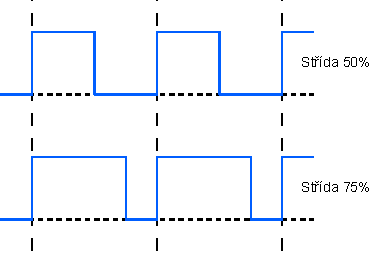
\includegraphics[scale=1]{obrazky-figures/pwm_duty_cycle.pdf}
	\caption{Signál pro různé hodnoty střídy}
	\label{}
\end{figure}

\subsubsection*{DC Motor}
%vysvětlit jak dc motor funguje ?
Dc motor má stator, permanentní magnet. A rotor, cívky do kterých se pak posílá proud tak aby se od statoru odpuzovaly a roztáčí se tak rotor.
%L298 - bere vetsi proud, obrazek se schematem (full bridge)

\subsubsection*{Led}

\subsubsection*{Servo}
Adeept AWD 4WD využívá pouze jedno servo, a to na ovládání úhlu kamery. Konkrétně se jedná o model Adeept AD002. Je ovládané pomocí PWM signálu. Generování tohoto signálu zajišťuje čip PCA9685 který je umístěný na Robot HAT.

\subsubsection*{Camera}

\subsubsection*{Depth module}
%hc-sr04
Funguje na principu radaru. Vyšle zvukovou vlnu na frekvenci 40Khz %je v tutorialu adeept
 a uloží si časovou značku. Následně poslouchá než se mu vlna vrátí a tehdy uloží druhou značku. Kdyz pak ví jak rychle se šíří zvuk ve vzduchu dokáže vypočítat vzdálenost od překážky.

$$S = (T_2 - T_1) * V_S / 2$$
Kde $T_1$ je moment kdy byla vyslána vlna $T_2$ kdy byla vlna přijata a $V_S$ rychlost šíření zvuku ve vzduchu.

\subsubsection*{Line tracking}
Funguje podobne jako depth module. Vysílá ultračervené tentokrát světlo a sleduje jestli došlo k odrazu. Bílý papír většinu světla odrazí a senzor jej zachytí, naopak černá čára světlo pohltí a senzor tak pozná že našel čáru.

\section{Aktuální software}

%koncepce (multithreading, knihovny)

\


%zhodnocení (plánované změny a naopak ponechané části)

\section{Seznámení s ROS2}
Práce je implementovaná s použitím ros2 verze iron.
%ideas that migt or might not be included
%ros1
%workspace

\subsection*{Koncepty}


\subsubsection*{Node} %prepsat aby to bylo stylisticky hezci
Celý ROS2 systém se skládá z určitého počtu těchto uzlů, které mezi sebou navzájem komunikují. ROS2 si zakládá na objektovém přístupu a implementačně je Node objekt který dědí ze třídy Node. 
%iterative execution
%other node functions

\subsubsection*{Topic}
Je základním a také nejčastěji používaným způsobem pomocí kterého ROS2 Node mezi sebou komunikují. Topic je přesně pojmenované místo, do kterého může n uzlů posílat data (Publish) a m poslouchat co bylo posláno (Subscribe). Zprávy posílané do topicu mají přesně daný formát a jsou posílány asynchronně. Typickým příkladem použití může být topic, do nějž posílá data uzel ovládající kameru a několik dalších uzlů které tyto data potřebují jej mohou číst. \cite{ros2_introduction}

\subsubsection*{Service}
Sevice funguje stejně jako klasická komunikace přes počítačovou síť klient -- server. Jedná se tedy o synchronní komunikaci kde jedna node poskytuje nějakou službu a ostatní si na ni mohou poslat požadavek. Od service se typicky předpokládá okamžitá odpověď aby nedošlo k narušení (control cycle) volající node. \cite{ros2_introduction}


\subsubsection*{Action} %cite web documentation
Jedná se o rozšířenou verzi service. Akce z pravidla vykonává déle trvající požadavek. Například provedení řídícího manévru robota, který je prováděn v reálném světě a jeho provedení není tedy krátkodobá záležitost. Akce pak na rozdíl od service dokáže v průběhu vykonávání této činnosti odesílat průběžné aktualizace o aktuálním stavu provádění zpět volající node. Implementačně funguje akce jako dva service a jeden topic. Cílový (goal) service slouží k zaslání požadavku na server a jeho potvrzení. Výsledkový (result) pak vrací výsledek operace. V průběhu akce pak server posílá aktualizace do topicu.

\subsubsection*{Interface}
Interface udává přesný formát jednotlivých zpráv, které jsou posílány mezi uzly.
Definice jedné datové položky pak vypadá následovně: datový\_typ název (int8 speed).
Existují tři %check if this is true
druhy souborů, které slouží k definici těchto zpráv. Prvním jsou .msg zprávy, ty jsou používány v topicu a obsahují pouze seznam položek, které jsou posílány. Druhým je service, který obsahuje dvě části, požadavek a odpověď, každá je tvořena seznamem položek a jsou odděleny řadkem s \verb|---|. Poslední je action, které se skládají ze tří seznamů, jeden pro požadavek, druhý pro odpověd a poslední pro aktualizace o stavu zprávy.

\subsubsection*{Parametry} %revisit after i use this in code
Ros2 uzly umí používat parametry, aby bylo možné jim předat hodnoty při spuštění a nemusely být uloženy ve zdrojových kódech. Typicky se přes parametry předávají cesty ke konfiguračním souborům. 

\subsubsection*{Launch File} %revisit after i do this properly
Protože každý ros2 uzel by měl mít za úkol jednu jednoduchou úlohu a celý systém se skládá z velkého množství propojených a komunikujících uzlů, stává se spouštění všech uzlů zvláště zdlouhavým. Proto existují launch soubory, které definují které uzly spustit, v jakém namespace a s jakými parametry. Launch soubory lze volat z jiných lauch souborů. %explain the structure here (package, higher level) 

\subsection*{Knihovny}




\chapter{Implementace} %prejmenovat, hodne todo, vetsina neni naimplementovana
\section{Struktura kódu}
\section{Manuální řízení}
\section{Sledování čáry}

\chapter{Závěr}
%cca strana


%===============================================================================

% Pro kompilaci po částech (viz projekt.tex) nutno odkomentovat
%\end{document}
